\documentclass[fleqn,10pt]{wlscirep}
\usepackage[utf8]{inputenc}
\usepackage[T1]{fontenc}
\usepackage{lineno}
\graphicspath{{./img/}{./pictures/}{./images/}}
\linenumbers

%in the preamble
%--------------------------------
\usepackage{natbib}
\bibliographystyle{jabbr}
%--------------------------------

\title{Data Descriptor Title (110 character maximum, inc. spaces)}

\author[1,2]{Yuhang Lin}
\author[1,2]{Heike Hofmann}

\affil[1]{Iowa State University, Department of Statistics, Ames, }
\affil[2]{Center for Statistics and Applications in Forensic Evidence
(CSAFE), Iowa State University, Ames, }

\affil[*]{corresponding author(s): Yuhang
Lin (yhlin@iastate.edu) {\color{red} ????????it.corresponding returns nothing} }
\affil[*]{corresponding author(s): Heike
Hofmann (hofmann@iastate.edu) {\color{red} ????????it.corresponding returns nothing} }

\begin{abstract}
\textcolor{gray}{(maximum 170 words) This is a manuscript template for Data Descriptor submissions to \emph{Scientific Data} (\href{http://www.nature.com/scientificdata}{http://www.nature.com/scientificdata}). The abstract must be no longer than 170 words, and should succinctly describe the study, the assay(s) performed, the resulting data, and the reuse potential, but should not make any claims regarding new scientific findings. No references are allowed in this section.}
\end{abstract}
\begin{document}

\flushbottom
\maketitle
%  Click the title above to edit the author information and abstract

\thispagestyle{empty}

\noindent \textcolor{gray}{Please note: Abbreviations should be introduced at the first mention in the main text – no abbreviations lists or tables should be included. Structure of the main text is provided below.}

\section*{Background \& Summary}

\textcolor{gray}{(unlimited length) An overview of the study design, the assay(s) performed, and the created data, including any background information needed to put this study in the context of previous work and the literature. The section should also briefly outline the broader goals that motivated the creation of this dataset and the potential reuse value. We also encourage authors to include a figure that provides a schematic overview of the study and assay(s) design. The Background \& Summary should not include subheadings. This section and the other main body sections of the manuscript should include citations to the literature as needed.}

\section*{Methods}

In this study, aluminum wire was used to create an optimal scenario
where the most amount of information could be transferred from the tool
to the substrate, despite the wire in James Genrich's case being made of
lead. The aluminum wire used was 16 Gauge/1.5 mm, anodized.

To cut the wire, 4-inch pieces were unspooled and cut using Kaiweets
wire cutters, model KWS-105, as shown in Figure
\ref{fig: kaiweet-label}, for 1 blade location, either inner, middle, or
outer, which gives us 1 replicate. Each piece was then cut into half to
create 2-inch pieces for each side, AB and CD, with a sharpie line
marking the cut ends, giving us 4 samples. Both AB and CD sides form
tent structures, as shown in Figure \ref{fig: x3p_tent}, and we can
separate each side of the tent into 2 pieces, as shown in Figure
\ref{fig: T1W}, resulting in 8 scans. We repeated this process for all 3
locations along the blade and 5 wire cutters, with 2 replicates for each
tool-edge-location combination, resulting in 120 scans. Each piece was
labeled with the naming conventions, T(ool) 1/2/3/4/5 (Edge) A/B/C/D
W(ire) - L(ocation) I(nner)/M(iddle)/O(uter) - R(epetition) 1/2, with
T1AW-LI-R1 being the piece cut by tool 1 on the A edge at the inner
location for the first repetition.

A more detailed procedure, including standard scanning protocols for the
confocal microscope in Figure \ref{fig: wire-microscope}, can be found
in the
\href{https://github.com/heike/Wirecuts/blob/main/README.md}{README of the GitHub repository \texttt{heike/Wirecuts}}
\textcolor{red}{(High-res pics needed in the README)}. The scanned
surfaces are saved in a resolution of \(0.645 \mu m \times 0.645 \mu m\)
per square pixel in an \texttt{x3p} file format.

\begin{figure}[ht]
\centering
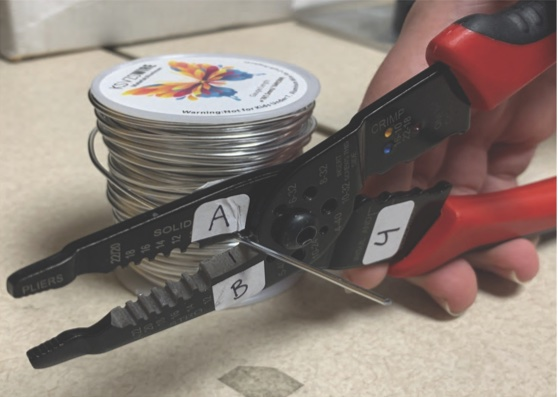
\includegraphics[width=0.5\linewidth]{kaiweet-label.jpg}
\caption{Legend (350 words max). Example legend text.}
\label{fig: kaiweet-label}
\end{figure}

\begin{figure}[ht]
\centering
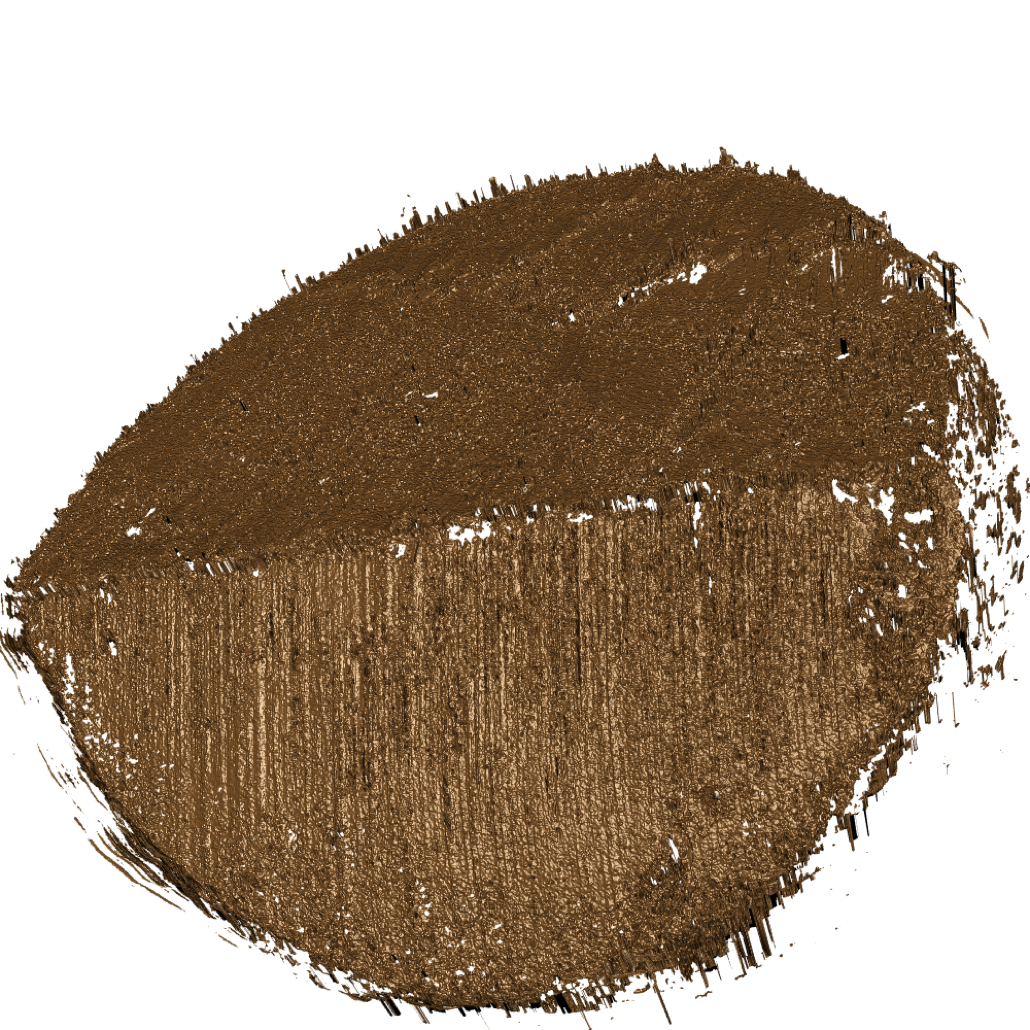
\includegraphics[width=0.25\linewidth]{x3p_tent.png}
\caption{Legend (350 words max). Example legend text.}
\label{fig: x3p_tent}
\end{figure}

\begin{figure}[ht]
\centering
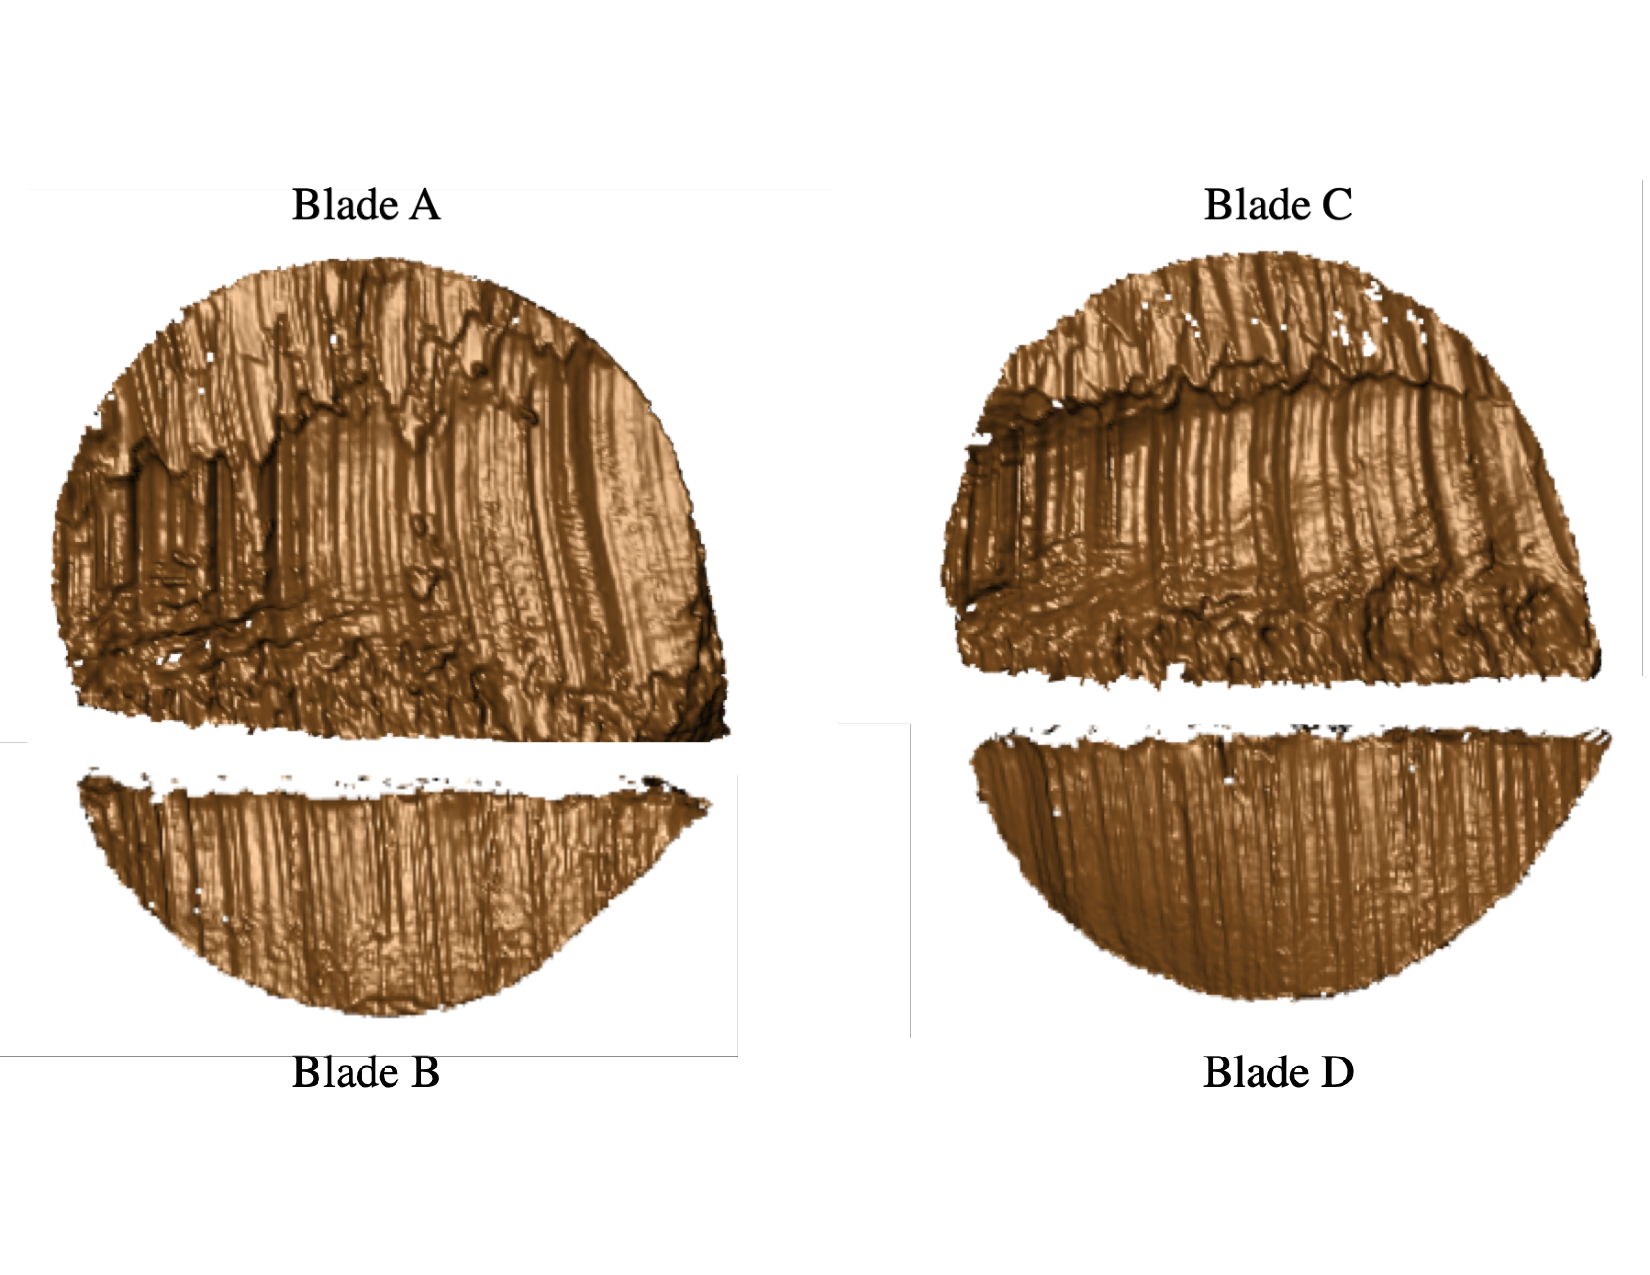
\includegraphics[width=0.5\linewidth]{T1W.pdf}
\caption{Legend (350 words max). Example legend text.}
\label{fig: T1W}
\end{figure}

\begin{figure}[ht]
\centering
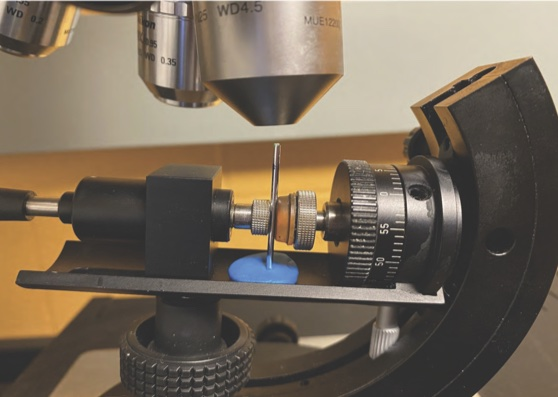
\includegraphics[width=0.5\linewidth]{wire-microscope.jpg}
\caption{Legend (350 words max). Example legend text.}
\label{fig: wire-microscope}
\end{figure}

\textcolor{gray}{(unlimited length) The Methods should include detailed text describing any steps or procedures used in producing the data, including full descriptions of the experimental design, data acquisition assays, and any computational processing (e.g. normalization, image feature extraction). See the detailed section in our submission guidelines for advice on writing a transparent and reproducible methods section. Related methods should be grouped under corresponding subheadings where possible, and methods should be described in enough detail to allow other researchers to interpret and repeat, if required, the full study. Specific data outputs should be explicitly referenced via data citation (see Data Records and Citing Data, below).}

\textcolor{gray}{Authors should cite previous descriptions of the methods under use, but ideally the method descriptions should be complete enough for others to understand and reproduce the methods and processing steps without referring to associated publications. There is no limit to the length of the Methods section. Subheadings should not be numbered.}

\textcolor{gray}{Authors should review the transparent methods checklist below, and ensure that their manuscript complies with any relevant points. Authors are also encouraged to search FAIRsharing.org for community reporting standards that may be relevant to their specific data-type.}

Transparent Methods Checklist

\begin{itemize}
  \item
  Materials \& reagents:
  Identify commercial suppliers of reagents, instrumentation or kits, when the source is critical to the outcome of the experiments.
  Declare any restrictions on the availability of unique materials (more information here).
  Provide catalogue or clone numbers for all antibodies (if available). For primary antibodies, provide proof of validation for the relevant species and applications.
  
  \item
  Exclusion criteria: If any data or samples were excluded, explain the exclusion criteria and state in the methods whether the criteria were established before the study was conducted.
  
  \item
  Randomization \& blinding: For any studies that involve assigning samples, animals or participants into different groups:
  State clearly whether randomization methods were used. If randomization was not employed, this should be clearly stated.
  State clearly whether blinding was employed during data collection. If blinding was not employed, this should be clearly stated.
  
  \item
  Animal \& human studies (full journal policies here):
  Experiments involving human participants must identify the committee approving the experiments, and include a statement confirming that informed consent was obtained from all participants.
  Studies employing nonhuman animals should ensure that methods descriptions comply with the ARRIVE checklist.
  
  \item
  Cell lines:
  For each eukaryotic cell line used, state the source and whether the cell line has been authenticated or otherwise tested for integrity.
  If any commonly misidentified cell lines were used (see ICLAC or NCBI Biosample), justify their use.
  Report whether the cell lines were tested for mycoplasma contamination.
  
  \item
  Chemistry \& materials science: Manuscripts describing chemical syntheses, or characterizing new chemicals or materials should refer to the guidance at Nature Chemistry.
  
\end{itemize}

\section*{Data Records}

The complete data set is available on the ISU DataShare repository at
\href{https://iastate.figshare.com/}{https://iastate.figshare.com/},
which is public and open access for every interested researcher. The
data set consists of 120 scans in the \texttt{x3p} file format with the
naming convention as described before.
\textcolor{red}{Explain the x3p header info to some extent? x3ptools?}

\textcolor{gray}{(unlimited length) The Data Records section should be used to explain each data record associated with this work, including the repository where this information is stored, and to provide an overview of the data files and their formats. Each external data record should be cited numerically in the text of this section, for example \cite{Hao:gidmaps:2014}, and included in the main reference list as described below. A data citation should also be placed in the subsection of the Methods containing the data-collection or analytical procedure(s) used to derive the corresponding record. Providing a direct link to the dataset may also be helpful to readers (\hyperlink{https://doi.org/10.6084/m9.figshare.853801}{https://doi.org/10.6084/m9.figshare.853801}).}

\textcolor{gray}{Tables should be used to support the data records, and should clearly indicate the samples and subjects (study inputs), their provenance, and the experimental manipulations performed on each (please see 'Tables' below). They should also specify the data output resulting from each data-collection or analytical step, should these form part of the archived record.}

\section*{Technical Validation}

For the data collection process, two team members did the cutting and
labeling together, then one person did the scanning and named according
to the naming convention above. The scanning was done in a specific
order to ensure consistency across all scans. The data was saved in a
consistent format to ensure that they could be easily accessed and
analyzed. A third person then checked the data to ensure that the data
was consistent in naming and accurate.

We also conduct numerical comparisons between 2 replicates made by the
same side of the same tool at the same location. For example, we compare
T1AW-LI-R1 to T1AW-LI-R2, T1BW-LI-R1 to T1BW-LI-R2, and so on, as shown
in Figure \ref{fig: scans_pair}. The comparison is done by aligning the
two scans and the cross-correlation function (CCF) between the two
scans.
\textcolor{red}{Explain the manual extraction in details? explain striations, profiles, signals, etc?}
We know that signals from two replicates with the same
tool-edge-location combination should yield similar signals, which
results in high CCF values close to 1, and the values we got in Figure
\ref{fig: signals_pair_alignment} achieve our expectation. For
validation of all other pairs of scan replicates, see the detailed
\href{https://heike.github.io/Wirecuts/data-descriptor/Technical_Validation.html}{report}.

\begin{figure}[ht]
\centering
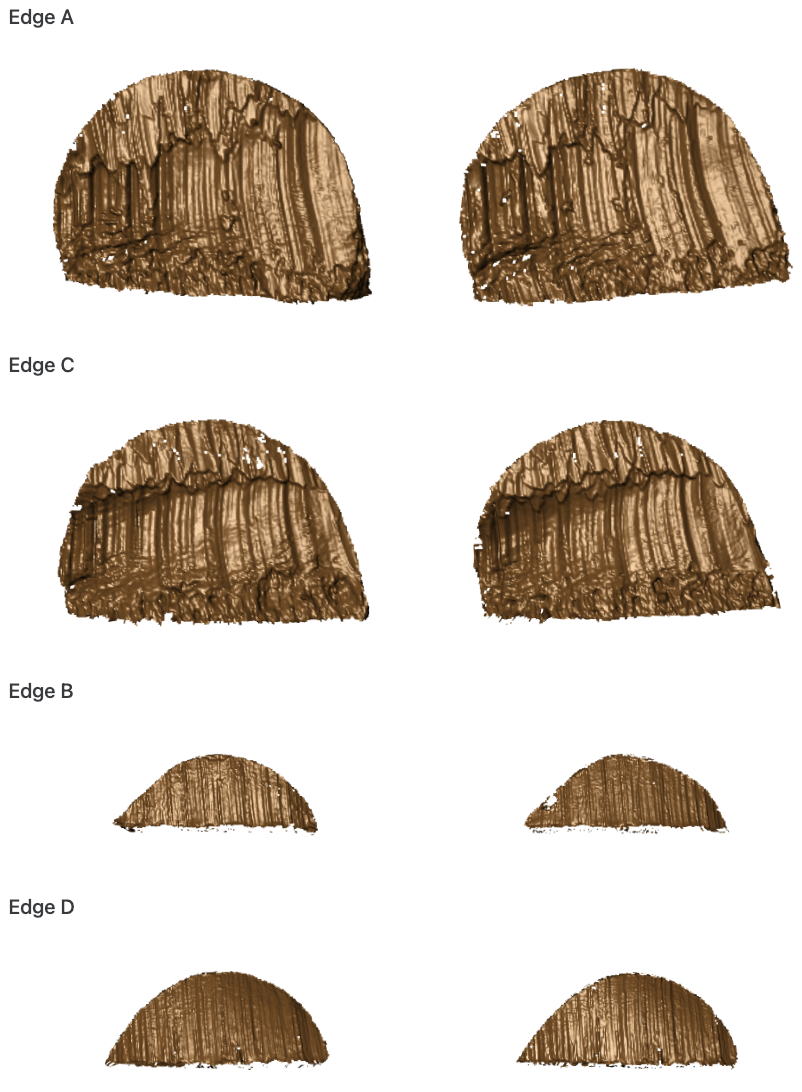
\includegraphics[width=0.8\linewidth]{scans_pair.png}
\caption{Legend (350 words max). Example legend text.}
\label{fig: scans_pair}
\end{figure}

\begin{figure}[ht]
\centering
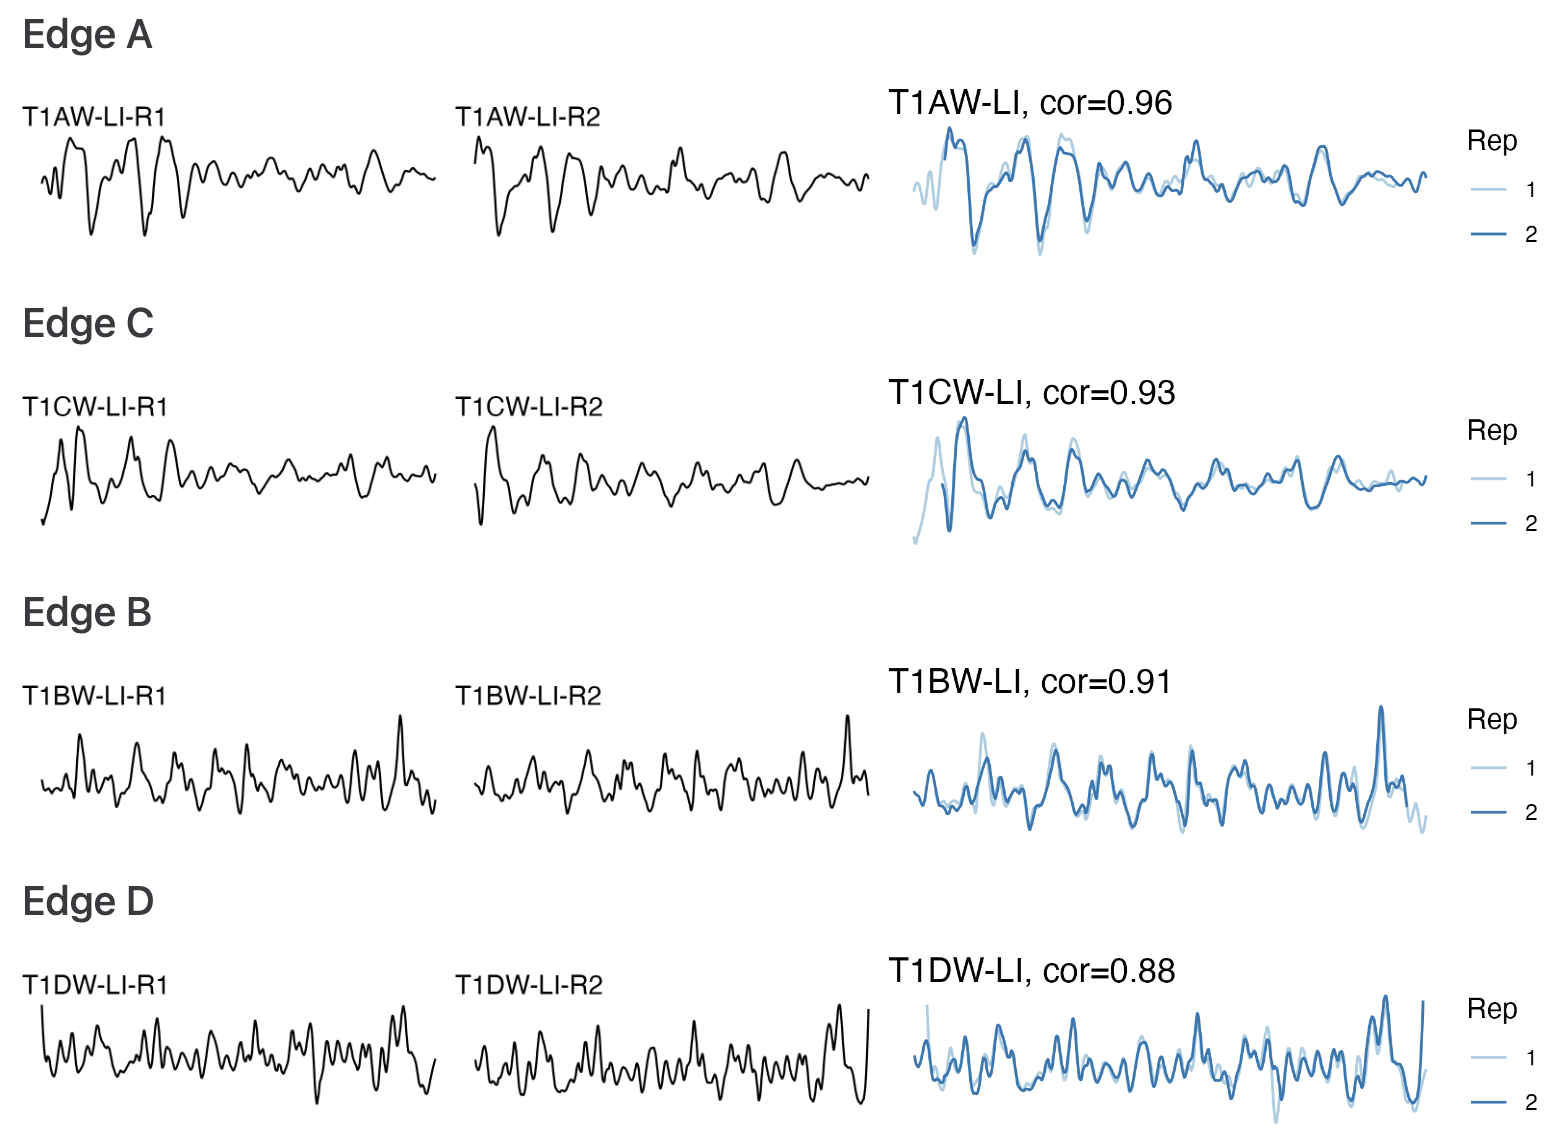
\includegraphics[width=0.8\linewidth]{signals_pair_alignment.png}
\caption{Legend (350 words max). Example legend text.}
\label{fig: signals_pair_alignment}
\end{figure}

\textcolor{gray}{(unlimited length) This section presents any experiments or analyses that are needed to support the technical quality of the dataset. This section may be supported by figures and tables, as needed. This is a required section; authors must present information justifying the reliability of their data.}

\begin{itemize}
  \item
  Measurement of data quality?
  
  \begin{itemize}
    \item
    Numeric measurements / tests: ?
    
    \item
    Visualizations: ?
    
    \item
    Check with existing data: ?
    
    \item
    Questionable / slur procedures:
      
      \begin{itemize}
      \item
      \href{https://www.nature.com/articles/s41597-024-03341-w?_gl=1*5ya8g2*_up*MQ..&gclid=EAIaIQobChMInOXO84DVhgMViewWBR3vWQJAEAAYASAAEgJICfD_BwE#Sec28}{AidData’s Geospatial Global Chinese Development Finance Dataset}: \textcolor{gray}{Second, all data collected is reviewed by at least two individuals. Although this is not a double-blind review procedure, the use of satellite imagery to verify project locations results in far less uncertainty when compared to previous approaches to geocoding where locations were selected entirely based on text descriptions.}
      
      \item
      \href{https://www.nature.com/articles/s41597-024-03021-9?_gl=1*1u1zppx*_up*MQ..&gclid=EAIaIQobChMInOXO84DVhgMViewWBR3vWQJAEAAYASAAEgJICfD_BwE#Sec9}{A large open access dataset of brain metastasis 3D segmentations on MRI with clinical and imaging information}: \textcolor{gray}{A medical student (D.R.) double checked and adjusted the revised NIfTI segmentation masks and manually counted the number of lesions with contrast-enhancement, necrosis, and peritumoral edema for each patient.}
      
      \item
      \href{https://www.nature.com/articles/s41597-024-03445-3?_gl=1*1ikco52*_up*MQ..&gclid=EAIaIQobChMInOXO84DVhgMViewWBR3vWQJAEAAYASAAEgJICfD_BwE#Sec11}{Time series of freshwater macroinvertebrate abundances and site characteristics of European streams and rivers}: \textcolor{gray}{Technical validation of the TREAM dataset was achieved through exclusion of time series data that did not match our inclusion criteria and data standardisation steps (outlined in Methods above). Any noted issues that did not adhere to the outlined standardisation within the datasets from the 41 independent projects included in this dataset were checked with data providers and corrected or removed when standardisation was not achievable (e.g., when collection methods changed over the course of the time series).}
      
      \item
      \href{https://www.nature.com/articles/s41597-023-02684-0?_gl=1*1t69zgo*_up*MQ..&gclid=EAIaIQobChMInOXO84DVhgMViewWBR3vWQJAEAAYASAAEgJICfD_BwE#Sec12}{3D surgical instrument collection for computer vision and extended reality}: \textcolor{gray}{The main issue...Since we store our models in a standard format (STL), they are compatible with a large variety of visualisation and processing software.}
      
      \item
      \href{https://www.nature.com/articles/s41597-024-03396-9?_gl=1*1ikco52*_up*MQ..&gclid=EAIaIQobChMInOXO84DVhgMViewWBR3vWQJAEAAYASAAEgJICfD_BwE#Sec4}{Three-dimensional reconstruction of high latitude bamboo coral via X-ray microfocus Computed Tomography
}: \textcolor{gray}{Regular quality assurance inspections are carried out on the µ-CT scanner to verify its metrological and geometrical (alignments) accuracy for conducting the scans. The geometry of source to object and source to detector distances are verified whenever there is any significant physical interaction with the source such as re-alignment, change of filament, or source anode change. This calibration process involves scanning a specially designed phantom known as an ‘hourglass’36, which consists of three pairs of high-sphericity spheres. The sphere sizes are as follows: two spheres with a diameter of 3.000 mm, two spheres with a diameter of 6.000 mm, and two spheres with a diameter of 9.525 mm, and each sphere is kept in contact with its size-counterpart. By using this phantom, it becomes possible to accurately determine a known distance, specifically the centre-to-centre distance of the spheres, in a threshold-independent manner. If the measured distance deviates beyond the acceptable limits of metrological accuracy, the system’s calibration parameters are adjusted to ensure agreement between the measured distance and the actual distance.}
      
      \end{itemize}
      
    \end{itemize}
  
\end{itemize}

\section*{Usage Notes}

The data set can be easily accessed with the \texttt{CRAN} \texttt{R}
package \texttt{x3ptools}. Further analysis can be conducted with the
\texttt{GitHub} \texttt{R} package \texttt{wire} and the \texttt{GitHub}
\texttt{R} shiny app \texttt{wireShiny}. We already conduct
between-replicate comparisons in the technical validation section, and
we can also conduct across-replicate comparisons to establish error
rates threshold and produce other analysis plots. The resulting CCFs are
shown in the boxplot in Figure \ref{fig: ccf_boxplot}. We can see that
the CCF values for the same sources are close to 1, while the CCF values
for different sources are much lower. This difference can be used to
establish a threshold for CCF and help us draw conclusion about the
similarity between wire cut scans, which can be used in real crime
scenes. The density plot in Figure \ref{fig: ccf_density} shows the
distribution of the CCF values. The overlapping points between the two
distributions can be a rough threshold. The receiver operating
characteristic (ROC) curve in Figure \ref{fig: ccf_ROC} shows the true
positive rate against the false positive rate, gives us a true threshold
of 0.589 to control the false positive rate (FPR) to be less than 0.05,
and 0.658 to control the FPR to be less than 0.01.

\begin{figure}[ht]
\centering
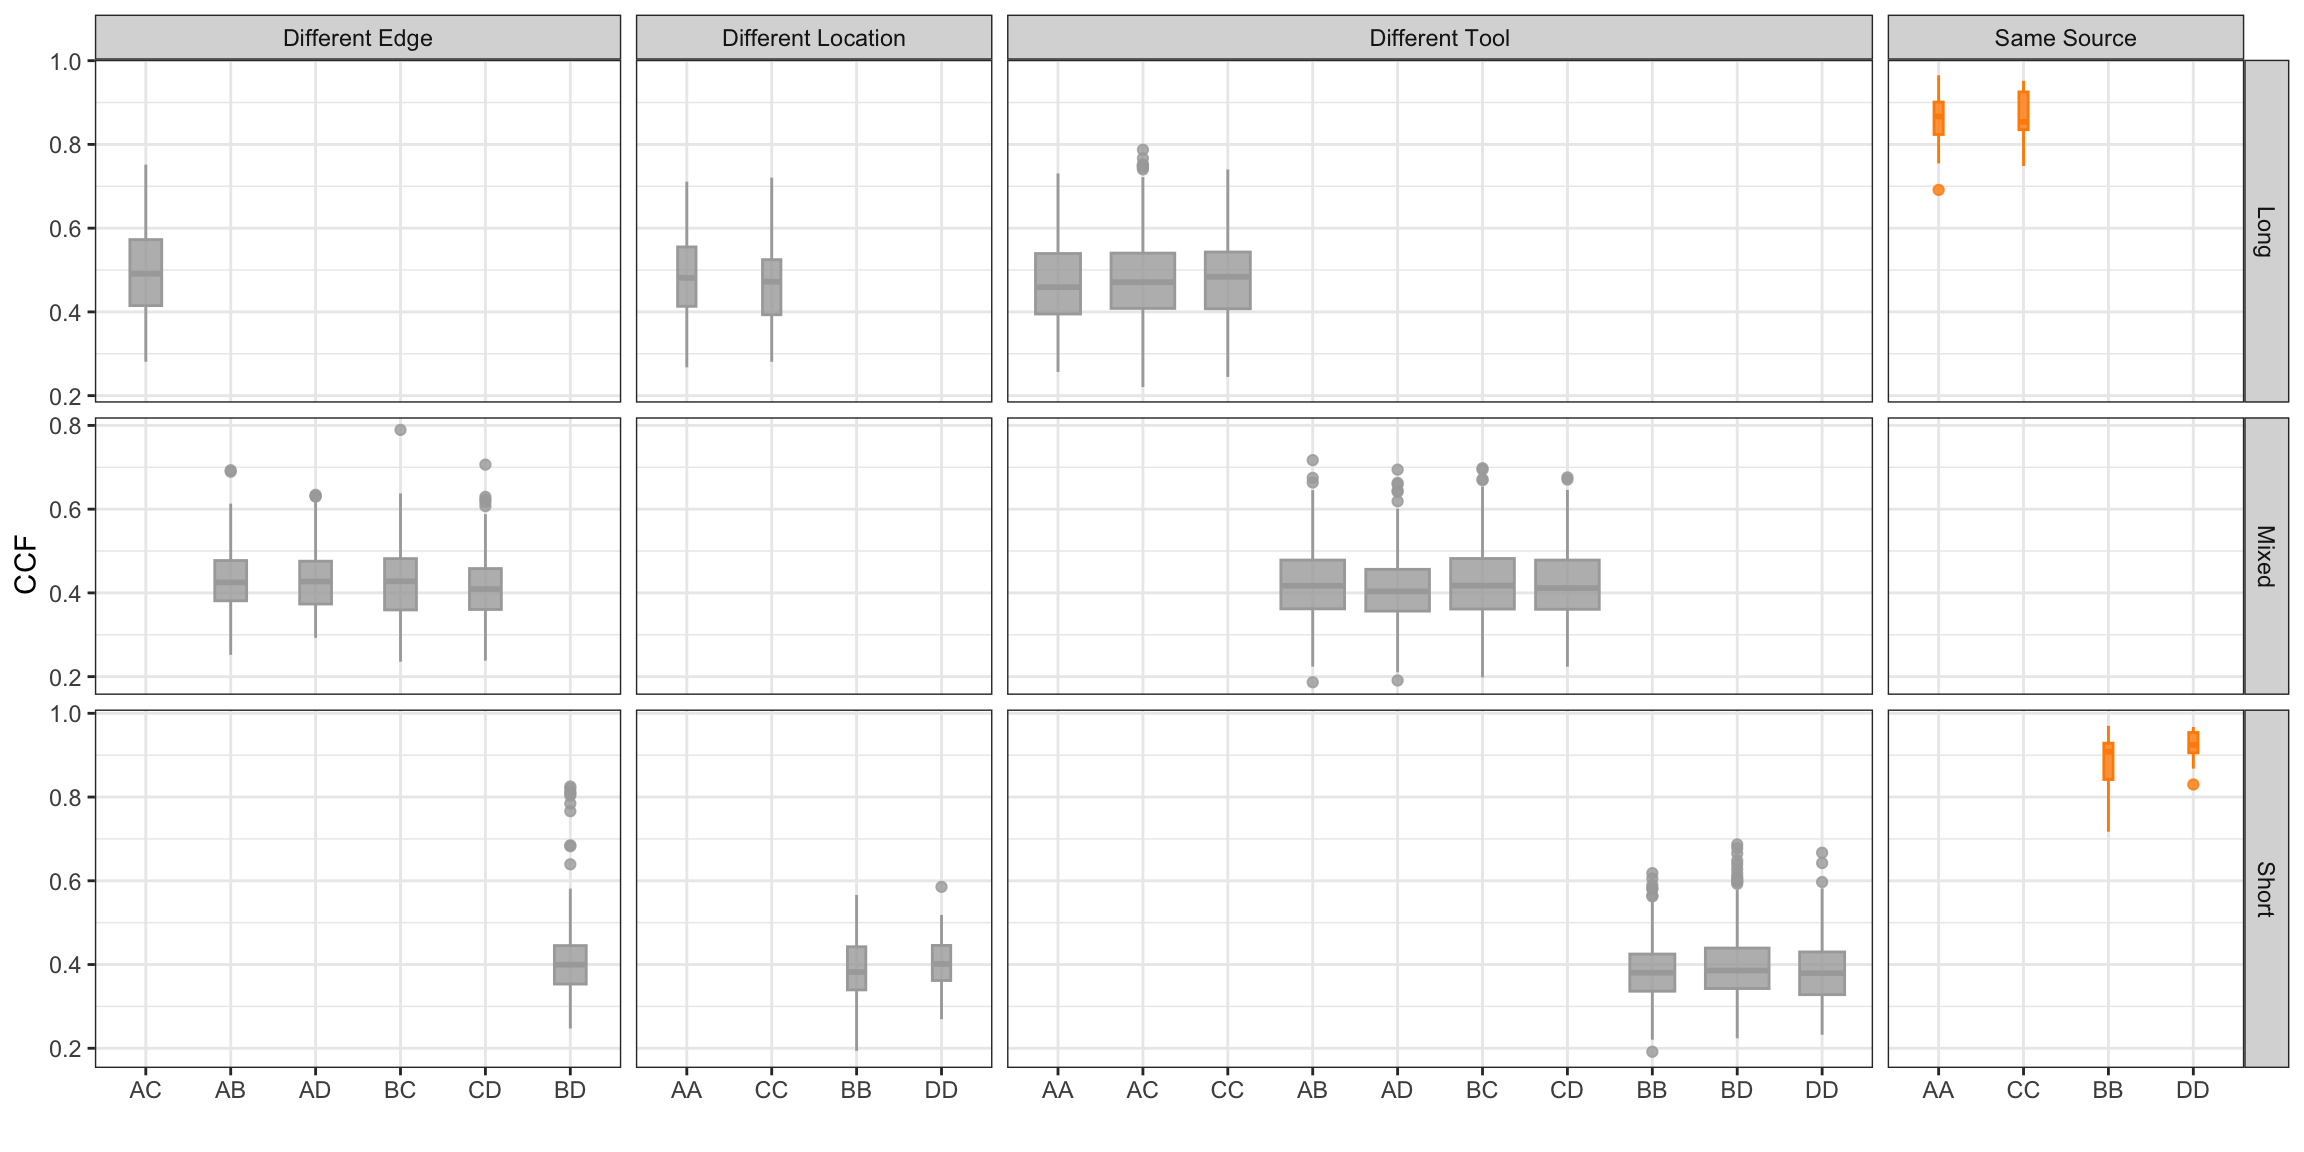
\includegraphics[width=0.8\linewidth]{ccf_boxplot.png}
\caption{Legend (350 words max). Example legend text.}
\label{fig: ccf_boxplot}
\end{figure}

\begin{figure}[ht]
\centering
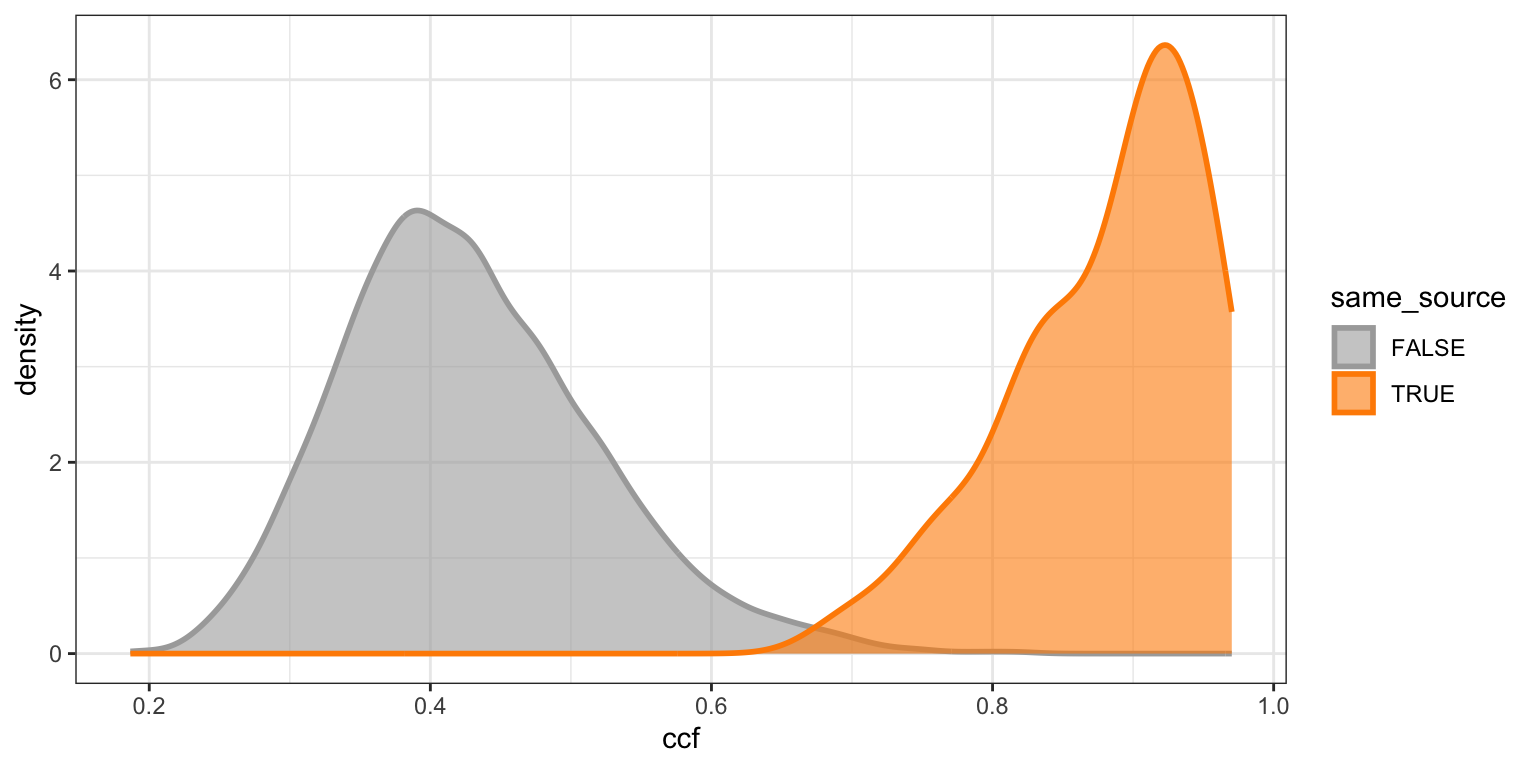
\includegraphics[width=0.8\linewidth]{ccf_density.png}
\caption{Legend (350 words max). Example legend text.}
\label{fig: ccf_density}
\end{figure}

\begin{figure}[ht]
\centering
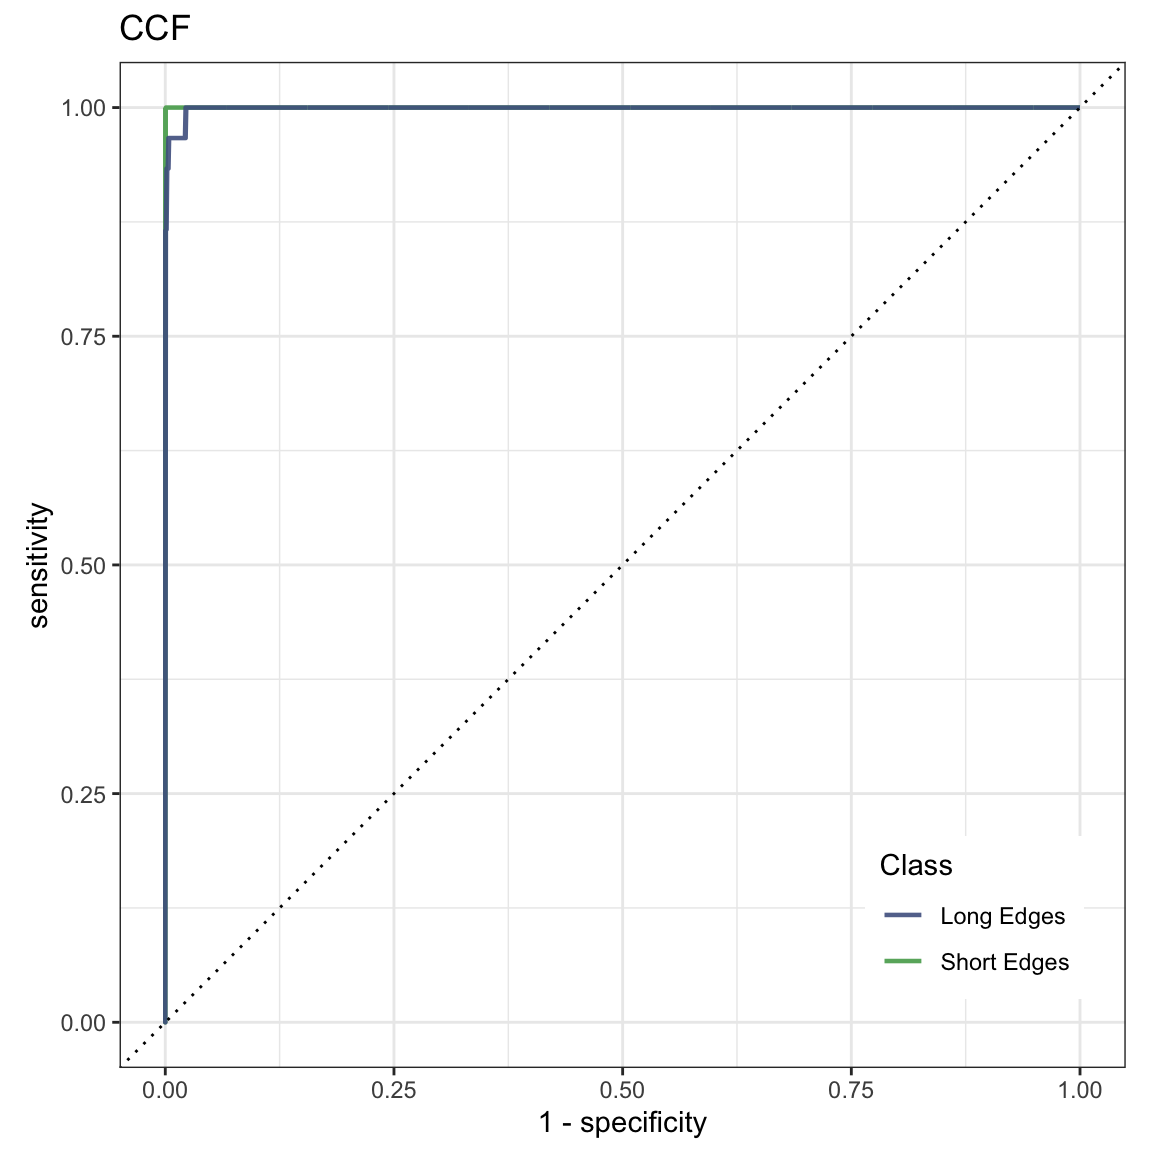
\includegraphics[width=0.5\linewidth]{ccf_ROC.png}
\caption{Legend (350 words max). Example legend text.}
\label{fig: ccf_ROC}
\end{figure}

\textcolor{gray}{(unlimited length) The Usage Notes should contain brief instructions to assist other researchers with reuse of the data. This may include discussion of software packages that are suitable for analysing the assay data files, suggested downstream processing steps (e.g. normalization, etc.), or tips for integrating or comparing the data records with other datasets. Authors are encouraged to provide code, programs or data-processing workflows if they may help others understand or use the data. Please see our code availability policy for advice on supplying custom code alongside Data Descriptor manuscripts.}

\textcolor{gray}{For studies involving privacy or safety controls on public access to the data, this section should describe in detail these controls, including how authors can apply to access the data, what criteria will be used to determine who may access the data, and any limitations on data use.}

\section*{Code availability}

\textcolor{gray}{For all studies using custom code in the generation or processing of datasets, a statement must be included under the heading "Code availability", indicating whether and how the code can be accessed, including any restrictions to access. This section should also include information on the versions of any software used, if relevant, and any specific variables or parameters used to generate, test, or process the current dataset.}

\section{End of Body}\label{end-of-body}

\textcolor{red}{Note that the bibliography style and the name of the bib-file are hard coded in the template file right now.}

\bibliography{references}

\noindent LaTeX formats citations and references automatically using the bibliography records in your .bib file, which you can edit via the project menu. Use the cite command for an inline citation, e.g. \cite{Kaufman2020, Figueredo:2009dg, Babichev2002, behringer2014manipulating}. For data citations of datasets uploaded to e.g. \emph{figshare}, please use the \verb|howpublished| option in the bib entry to specify the platform and the link, as in the \verb|Hao:gidmaps:2014| example in the sample bibliography file. For journal articles, DOIs should be included for works in press that do not yet have volume or page numbers. For other journal articles, DOIs should be included uniformly for all articles or not at all. We recommend that you encode all DOIs in your bibtex database as full URLs, e.g. https://doi.org/10.1007/s12110-009-9068-2.

\section*{Acknowledgements} 
Acknowledgements should be brief, and should not include thanks to
anonymous referees and editors, or effusive comments. Grant or
contribution numbers may be acknowledged.

\section*{Author contributions statement}

Y.L. did all of the work, H.H. made him do the work. But seriously, this
paper is the one where we need to cite everybody: Eden Amin, Curtis
Mosher, Jeff Salyards.
Must include all authors, identified by initials, for example:
A.A. conceived the experiment(s), A.A. and B.A. conducted the experiment(s), C.A. and D.A. analysed the results. All authors reviewed the manuscript. 

\section*{Competing interests} (mandatory statement)

The corresponding author is responsible for providing a
\href{https://www.nature.com/sdata/policies/editorial-and-publishing-policies#competing}{competing interests statement}
on behalf of all authors of the paper. This statement must be included
in the submitted article file. H.H. is a technical advisor to AFTE
(Association of Firearms and Toolmarks Examiners), fellow of the ASA
(American Statistical Association), and committee member of the ASA
Forensic Science Committee. H.H. has testified as court witness on
behalf of judge April Neubauer, NY State Supreme Court Criminal Term in
New York City.

% XXX Delete the section below later
\section*{Figures \& Tables}


Figures, tables, and their legends, should be included at the end of the document. Figures and tables can be referenced in \LaTeX{} using the ref command, e.g. Figure \ref{fig:stream} and Table \ref{tab:example}. 

Authors are encouraged to provide one or more tables that provide basic information on the main ‘inputs’ to the study (e.g. samples, participants, or information sources) and the main data outputs of the study. Tables in the manuscript should generally not be used to present primary data (i.e. measurements). Tables containing primary data should be submitted to an appropriate data repository.

Tables may be provided within the \LaTeX{} document or as separate files (tab-delimited text or Excel files). Legends, where needed, should be included here. Generally, a Data Descriptor should have fewer than ten Tables, but more may be allowed when needed. Tables may be of any size, but only Tables which fit onto a single printed page will be included in the PDF version of the article (up to a maximum of three). 

Due to typesetting constraints, tables that do not fit onto a single A4 page cannot be included in the PDF version of the article and will be made available in the online version only. Any such tables must be labelled in the text as ‘Online-only’ tables and numbered separately from the main table list e.g. ‘Table 1, Table 2, Online-only Table 1’ etc.

\begin{figure}[ht]
\centering
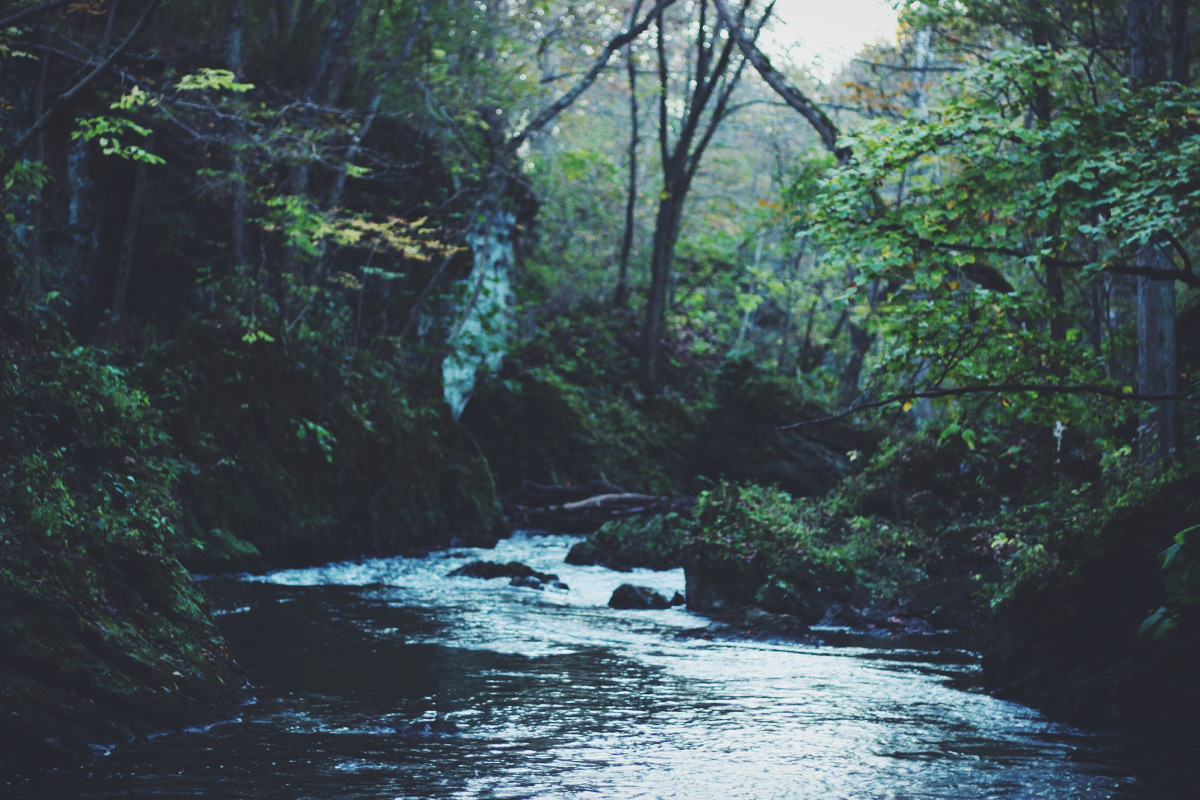
\includegraphics[width=\linewidth]{stream}
\caption{Legend (350 words max). Example legend text.}
\label{fig:stream}
\end{figure}

\begin{table}[ht]
\centering
\begin{tabular}{|l|l|l|}
\hline
Condition & n & p \\
\hline
A & 5 & 0.1 \\
\hline
B & 10 & 0.01 \\
\hline
\end{tabular}
\caption{\label{tab:example}Legend (350 words max). Example legend text.}
\end{table}

\end{document}
